% !TeX root = ../main.tex
% Add the above to each chapter to make compiling the PDF easier in some editors.

\chapter{Introduction}\label{chapter:introduction}
\section{Introduction to Sys-Sage Library}

High-Performance Computing (HPC) systems have undergone significant transformations, becoming increasingly complex. This complexity arises from the integration of various components, particularly the growing reliance on multi-core processors and \ac{GPU}s. As modern architectures evolve, understanding system behavior becomes more challenging, necessitating more sophisticated analysis tools.

Several approaches exist for analyzing system architectures, with one of the most commonly used tools being \texttt{hwloc}. This tool facilitates the construction of hardware topologies, mapping essential building blocks such as cores, caches, and \ac{NUMA} nodes. While \texttt{hwloc} provides fundamental insights into system topology and application scheduling, it is limited to \ac{CPU}-based static analysis.

However, contemporary architectures introduce dynamic resource allocation and isolation, rendering static analysis insufficient for comprehensive system evaluation. Consequently, dynamic analysis becomes increasingly valuable in modern computing environments. Given the growing dynamism of \ac{HPC} systems, a unified tool that consolidates the advantages of existing solutions while incorporating real-time hardware and resource utilization changes would be highly beneficial.

The \texttt{Sys-Sage} library addresses this need by offering a unified \ac{API} for accessing the state of modern architectures. As an \ac{open-source} solution, \texttt{Sys-Sage} is highly adaptable and supports the integration of diverse datasets, such as \ac{GPU} benchmarks and power efficiency metrics, enabling a comprehensive understanding of system performance. It constructs an internal representation of hardware topology alongside data paths, allowing for both \textbf{export} and, in future iterations, \textbf{import} capabilities to facilitate data storage and retrieval.

\section{Scope of This Work}

Currently, \texttt{Sys-Sage} provides support exclusively for \ac{C++}, limiting its accessibility to a broader audience. Meanwhile, \ac{Python} has emerged as the most widely used programming language, surpassing JavaScript with \textbf{16.925\%} of all GitHub projects developed in \ac{Python}\parencite{python-github-stats}. Given its widespread adoption, introducing a \ac{Python} \ac{API} for \texttt{Sys-Sage} would significantly enhance usability, enabling a larger community to leverage its capabilities.

The objective of this work is to develop a \ac{Python} interface for \texttt{Sys-Sage} while preserving the performance advantages of the underlying \ac{C++} implementation. This will be achieved by binding essential \ac{C++} library functions, allowing users to compile the code once and execute scripts efficiently with the compiled runtime.

The \ac{Python} \ac{API} must meet the following key requirements:
\begin{itemize}
    \item \textbf{Ease of installation} – Users should be able to set up the library with minimal effort.
    \item \textbf{User-friendliness} – The \ac{API} should offer an intuitive interface for seamless integration into \ac{Python}-based workflows.
    \item \textbf{High performance} – The binding should maintain the speed and efficiency of the original \ac{C++} implementation.
\end{itemize}

By achieving these objectives, this project will bridge the gap between \texttt{Sys-Sage}'s powerful analysis capabilities and the growing \ac{Python} developer community, fostering broader adoption and enhanced system analysis in \ac{HPC} environments.

\subsection{Acronyms}

Acronyms must be added in \texttt{main.tex} and are referenced using macros. The first occurrence is automatically replaced with the long version of the acronym, while all subsequent usages use the abbreviation.

For example: \texttt{\textbackslash ac\{TUM\}, \textbackslash ac\{TUM\}} $\Rightarrow$ \ac{TUM}, \ac{TUM}.

For more details, see the documentation of the \texttt{acronym} package\footnote{\url{https://ctan.org/pkg/acronym}}.

% \printbibliography

\section{Section}
Citation test~\parencite{latex}.


Acronyms must be added in \texttt{main.tex} and are referenced using macros. The first occurrence is automatically replaced with the long version of the acronym, while all subsequent usages use the abbreviation.

E.g. \texttt{\textbackslash ac\{TUM\}, \textbackslash ac\{TUM\}} $\Rightarrow$ \ac{TUM}, \ac{TUM}

For more details, see the documentation of the \texttt{acronym} package\footnote{\url{https://ctan.org/pkg/acronym}}.
\subsection{Subsection}

See~\autoref{tab:sample}, \autoref{fig:sample-drawing}, \autoref{fig:sample-plot}, \autoref{fig:sample-listing}.

\begin{table}[htpb]
  \caption[Example table]{An example for a simple table.}\label{tab:sample}
  \centering
  \begin{tabular}{l l l l}
    \toprule
      A & B & C & D \\
    \midrule
      1 & 2 & 1 & 2 \\
      2 & 3 & 2 & 3 \\
    \bottomrule
  \end{tabular}
\end{table}

\begin{figure}[htpb]
  \centering
  % This should probably go into a file in figures/
  \begin{tikzpicture}[node distance=3cm]
    \node (R0) {$R_1$};
    \node (R1) [right of=R0] {$R_2$};
    \node (R2) [below of=R1] {$R_4$};
    \node (R3) [below of=R0] {$R_3$};
    \node (R4) [right of=R1] {$R_5$};

    \path[every node]
      (R0) edge (R1)
      (R0) edge (R3)
      (R3) edge (R2)
      (R2) edge (R1)
      (R1) edge (R4);
  \end{tikzpicture}
  \caption[Example drawing]{An example for a simple drawing.}\label{fig:sample-drawing}
\end{figure}

\begin{figure}[htpb]
  \centering

  \pgfplotstableset{col sep=&, row sep=\\}
  % This should probably go into a file in data/
  \pgfplotstableread{
    a & b    \\
    1 & 1000 \\
    2 & 1500 \\
    3 & 1600 \\
  }\exampleA
  \pgfplotstableread{
    a & b    \\
    1 & 1200 \\
    2 & 800 \\
    3 & 1400 \\
  }\exampleB
  % This should probably go into a file in figures/
  \begin{tikzpicture}
    \begin{axis}[
        ymin=0,
        legend style={legend pos=south east},
        grid,
        thick,
        ylabel=Y,
        xlabel=X
      ]
      \addplot table[x=a, y=b]{\exampleA};
      \addlegendimage{empty legend}
      \addlegendentry{Example A}
      \addplot table[x=a, y=b]{\exampleB};
      \addlegendentry{Example B}
    \end{axis}
  \end{tikzpicture}
  \caption[Example plot]{An example for a simple plot.}\label{fig:sample-plot}
\end{figure}

\begin{figure}[htpb]
  \centering
  \begin{tabular}{c}
  \begin{lstlisting}[language=SQL]
    SELECT * FROM table WHERE tbl.str = "str"
  \end{lstlisting}
  \end{tabular}
  \caption[Example listing]{An example for a source code listing.}\label{fig:sample-listing}
\end{figure}

\begin{figure}[htpb]
  \centering
  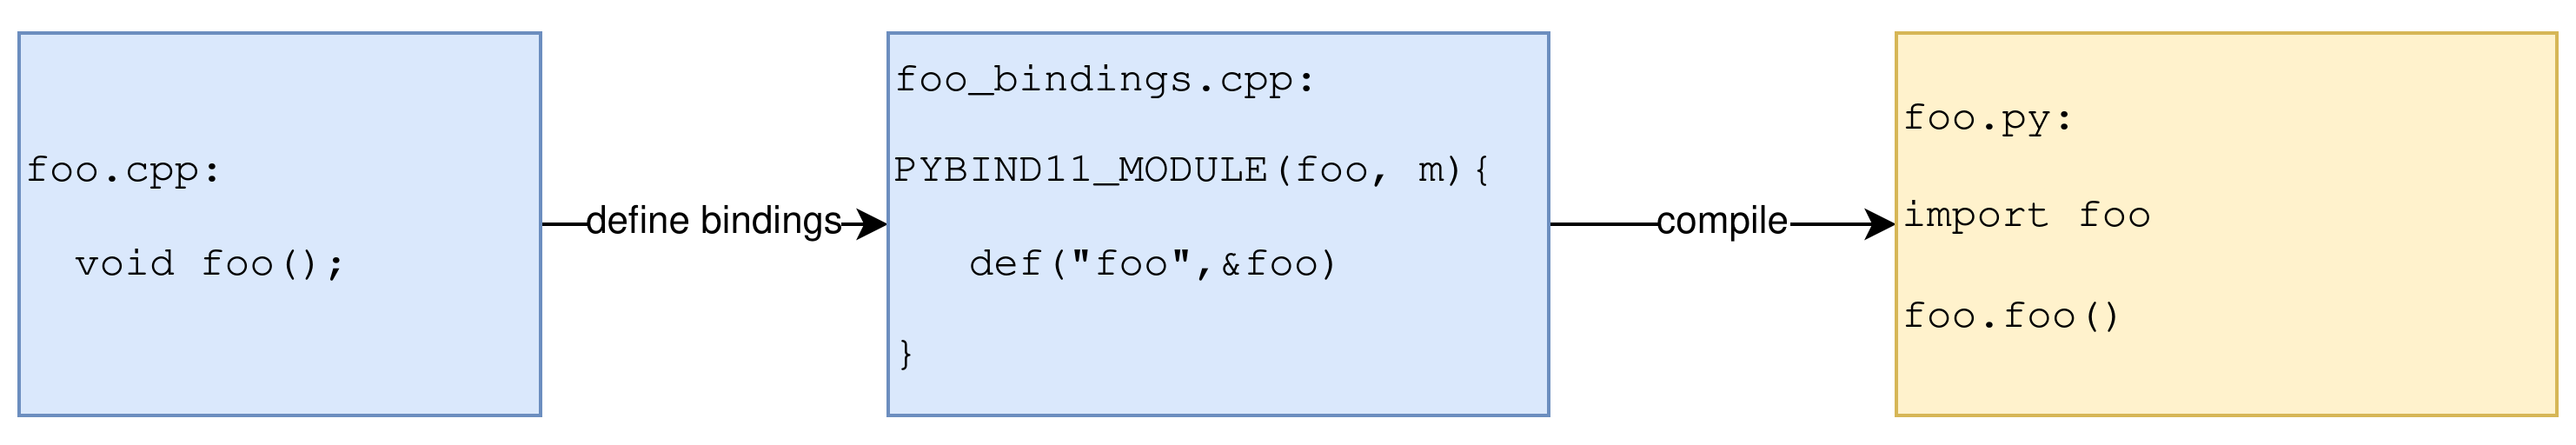
\includegraphics[width=\textwidth]{../figures/pybind_schema.png}
  \caption[Example image]{An example for a simple image.}\label{fig:sample-image}
\end{figure}


\begin{figure}[hptb]
    \centering
  
    \pgfplotstableset{col sep=&, row sep=\\}
    \pgfplotstableread{
      x & swig & pybind11 \\
      10 & 0.831514591 & 1.058577497 \\
      20 & 1.127118936 & 1.471500208 \\
      30 & 1.4772158 & 1.761273233 \\
      40 & 1.736514494 & 2.126912437 \\
      50 & 2.025210358 & 2.46362231 \\
      60 & 2.214553424 & 2.804167879 \\
      70 & 2.603474917 & 3.326882148 \\
      80 & 2.877264073 & 3.673826322 \\
      90 & 3.352056939 & 3.967651672 \\
      100 & 3.392421572 & 4.391185498 \\
      110 & 3.703171002 & 4.916812021 \\
      120 & 4.275075549 & 5.214867283 \\
      130 & 5.214835618 & 5.347268902 \\
      140 & 6.241614607 & 5.945904962 \\
      150 & 6.595369415 & 6.519765277 \\
      160 & 6.967670258 & 7.11302645 \\
      170 & 7.165744065 & 7.452702384 \\
      180 & 7.80374477 & 7.193507064 \\
      190 & 8.358989104 & 7.662745811 \\
      200 & 8.92708868 & 7.899299085 \\
      210 & 9.175657786 & 8.070269308 \\
      220 & 9.27380257 & 8.513974392 \\
      230 & 9.771330559 & 8.768865073 \\
      240 & 10.07812149 & 8.980851734 \\
      250 & 10.57007511 & 9.686946998 \\
      260 & 10.93630689 & 9.962699361 \\
      270 & 11.02586082 & 10.96497769 \\
      280 & 11.80790557 & 10.70239503 \\
      290 & 12.17019807 & 11.02871699 \\
      300 & 12.6979764 & 11.43657468 \\
    }\data
  
    \begin{tikzpicture}
      \begin{axis}[
          ymin=0,
          ymax=20,
          legend style={legend pos=north west},
          grid,
          thick,
          ylabel=Time (seconds),
          xlabel=Hierarchy depth
        ]
        \addplot+[mark=none] table[x=x, y=swig]{\data};
        \addlegendentry{SWIG -O3, shared-pointers}
        \addplot+[mark=none] table[x=x, y=pybind11]{\data};
        \addlegendentry{PyBind11 -O3, shared-pointers}
      \end{axis}
    \end{tikzpicture}
    \caption[Plot of SWIG and PyBind11 with shared-pointers]{A plot comparing the performance of SWIG and PyBind11 with optimization flag -O3 and shared-pointers.}\label{fig:swig-pybind11-shared-pointers-plot}
  \end{figure}
